\documentclass[11pt,letterpaper]{article}

\usepackage{../assets/scientific_report}
\usepackage{float}
\usepackage{listings}
\usepackage{xcolor}
\usepackage{graphicx}
\usepackage{geometry}

\geometry{headheight=23pt, top=2cm, bottom=2cm, left=2.5cm, right=2.5cm}
\setlength{\parskip}{0.5em}
\setlength{\parindent}{0pt}

\lstset{
    language=C,
    basicstyle=\ttfamily\small,
    keywordstyle=\color{blue}\bfseries,
    commentstyle=\color{green!60!black}\itshape,
    stringstyle=\color{red!80!black},
    numbers=left,
    numberstyle=\tiny\color{gray},
    numbersep=8pt,
    frame=single,
    breaklines=true,
    captionpos=b,
    tabsize=4,
    showstringspaces=false
}

\begin{document}
\pagestyle{plain}

\begin{center}
    {\LARGE\bfseries Coerência de Cache e Falso Compartilhamento}\\[0.4em]
    {\normalsize Eugenio Vitor Lopes dos Santos}\\[0.3em]
    {\small DCA3703, Programação Paralela, Universidade Federal do Rio Grande do Norte}\\[0.3em]
\end{center}

\section{Enunciado}

Implementar em C a estimativa estocástica de $\pi$ usando \texttt{rand()} para gerar os pontos. Cada thread deve usar uma variável privada para contar os acertos e acumular o total em uma variável global com \texttt{\#pragma omp critical}. Depois, implementar uma segunda versão em que cada thread escreve seus acertos em uma posição distinta de um vetor compartilhado. A acumulação deve ser feita em um laço serial após a região paralela. Comparar o tempo de execução das duas versões. Em seguida, substituir \texttt{rand()} por \texttt{rand\_r()} em ambas e comparar novamente. Explicar o comportamento dos quatro programas com base na coerência de cache e nos efeitos do falso compartilhamento.

\section{Fundamentação teórica}

\subsection{Método de Monte Carlo}

O quadrado $[-1,1] \times [-1,1]$ tem área $4$, e o círculo unitário inscrito tem área $\pi$. Sorteando pontos uniformes no quadrado e testando $x^2+y^2 \le 1$, a fração de acertos converge para a razão das áreas: $n_{dentro}/N \approx \pi/4$. A estimativa é $\hat{\pi}=4\cdot n_{dentro}/N$. O erro cai com $1/\sqrt{N}$, e o gerador define tanto a qualidade estatística quanto o custo computacional.

\subsection{\texttt{rand} com estado global contra \texttt{rand\_r} com estado privado}

O \texttt{rand()} guarda o estado em variável global oculta na libc. Cada chamada lê, atualiza e escreve esse estado. Com várias threads, sobram duas saídas ruins. Sem proteção, ocorre \textit{data race} e a sequência se corrompe. Com \texttt{critical}, a geração serializa e só uma thread gera por vez. A função \texttt{rand\_r(unsigned *seed)} recebe o estado por parâmetro. Se cada thread mantém \texttt{unsigned seed} local privada, cada uma avança sua própria sequência sem comunicação, e a geração paraleliza de verdade. Vetor de sementes contíguo \texttt{seeds[8]} reintroduz o problema: as sementes dividem a mesma linha de cache, e cada \texttt{rand\_r} invalida a linha dos vizinhos.

\subsection{\texttt{critical} por ponto contra privado mais redução serial}

A versão A usa contador privado \texttt{local} e uma única entrada em \texttt{critical} por thread: \texttt{total += local}. O custo de sincronização é de $P$ entradas, e o laço não tem tráfego coerente. A versão B com vetor escreve \texttt{hits[tid]++} no laço e soma em laço serial após a barreira. Se a escrita no vetor ocorre a cada acerto, há $N$ escritas concorrentes em posições vizinhas. A forma correta é manter a contagem privada durante o laço e realizar uma única escrita em \texttt{hits[tid]}, seguida de soma serial de $P$ elementos.

\subsection{Coerência de cache com caches privadas}

Cada núcleo só enxerga a RAM através de suas caches privadas L1/L2. Para manter a ilusão de memória única, o hardware controla a coerência por linha de $64$ B, com estados MESI e dois bits por linha: sujo e inválido. Em \textit{write-back}, o store escreve só na cache e marca $dirty=1$. O hardware só escreve na RAM na evicção ou quando outro núcleo pede a linha. Em \textit{write-through}, cada store atravessa até a memória. Quando um núcleo escreve em linha compartilhada, o hardware invalida as cópias nos vizinhos. O próximo load sofre miss e busca o valor novo. Uma variável compartilhada custa pouco para leitura ou escrita rara: basta copiar com \texttt{private} e \texttt{firstprivate}. Para escrita frequente, ela torna a cache inútil. Sem sincronização, há condição de corrida. Com \texttt{critical}, há serialização. Sem nenhum dos dois, há ping-pong de invalidações. No pior caso, o miss em linha suja remota custa dois acessos: o dono escreve a linha de volta, e o solicitante a busca em seguida.

\subsection{Falso compartilhamento}

A unidade de coerência é a linha, não a variável. Um vetor \texttt{long hits[8]} ocupa $64$ B e preenche exatamente uma linha de cache: oito contadores distintos disputam a mesma linha. Escritas em variáveis logicamente independentes invalidam-se mutuamente, e a linha pinga entre caches a cada iteração, mesmo sem compartilhamento lógico. A correção é afastar cada posição em $64$ B distintos com \textit{padding}: \texttt{struct \{ long v; char pad[56]; \} \_\_attribute\_\_((aligned(64)))}. Declarar \texttt{volatile}, trocar \textit{write-back} por \textit{write-through} ou envolver em \texttt{critical} não resolve: o primeiro não muda o layout, o segundo piora o tráfego, e o terceiro serializa.

\subsection{Snooping contra diretório}

Em \textit{snooping}, o hardware difunde cada miss ou escrita no barramento, e todas as caches espionam para ver se têm a linha. É \textit{broadcast} contínuo e não escala com dezenas de núcleos. No protocolo com diretório, um registro central junto à LLC guarda quem tem cada linha, e o hardware envia invalidação só a esses donos. O falso compartilhamento gera avisos inúteis nos dois casos, mas no \textit{snooping} o custo interrompe todos os nós.

\section{Implementação}

Foram avaliadas cinco versões em C11 com medição via \texttt{clock\_gettime(CLOCK\_MONOTONIC)} e controle de escopo com \texttt{default(none)}: v1 \texttt{critical+rand}, v2 \texttt{vetor+rand}, v3 \texttt{critical+rand\_r}, v4 \texttt{vetor+rand\_r} e v4-pad com \textit{slot} de $64$ B. Em v1 e v3, cada thread conta em \texttt{long local} e faz um único \texttt{\#pragma omp critical total += local}. Em v2 e v4, cada thread incrementa \texttt{hits[tid]} no laço quente para expor o falso compartilhamento, e a soma é serial após a região paralela. Em v3, v4 e v4-pad, a semente é local: \texttt{unsigned seed = 123456789U \^{} tid}. Compilação com GCC, \texttt{-std=c11 -O2 -Wall -fopenmp -lm}, $N=5.000.000$.

\newpage
\begin{lstlisting}[language=bash,caption={Compilação e execução}]
gcc -std=c11 -O2 -Wall -fopenmp v1_pi_critical_rand.c -o pi_critical_rand -lm
gcc -std=c11 -O2 -Wall -fopenmp v2_pi_vector_rand.c -o pi_vector_rand -lm
gcc -std=c11 -O2 -Wall -fopenmp v3_pi_critical_randr.c -o pi_critical_randr -lm
gcc -std=c11 -O2 -Wall -fopenmp v4_pi_vector_randr.c -o pi_vector_randr -lm
gcc -std=c11 -O2 -Wall -fopenmp v4_fix_pi_vector_randr_pad.c -o pi_vector_randr_pad -lm
OMP_NUM_THREADS=8 ./pi_critical_randr 5000000
OMP_NUM_THREADS=8 ./pi_vector_randr_pad 5000000
\end{lstlisting}

\section{Resultados e discussão}

Testes em Intel Core i7-14700HX sob WSL2 com 14 núcleos físicos e 28 threads lógicas, varredura de 1 a 28 threads com $N=5.000.000$. Cada ponto é a mediana de cinco repetições. As Figuras~\ref{fig:tempo} e \ref{fig:templog} mostram a curva completa em escala linear e em escala logarítmica, e a Figura~\ref{fig:barra} compara as cinco versões com 8 threads. O CSV completo com 28 linhas acompanha o relatório.

\begin{table}[H]
\centering
\caption{Tempo em segundos com $N=5.000.000$, varredura de 1 a 28 threads. Cada valor é a mediana de cinco repetições.}
\label{tab:tempos}
{\scriptsize
\begin{tabular}{crrrrr}
\hline
\textbf{Thr} & \textbf{v1 crit+rand} & \textbf{v2 vet+rand} & \textbf{v3 crit+rand\_r} & \textbf{v4 vet+rand\_r} & \textbf{v4-pad} \\ \hline
1 & 0,2010 & 0,2039 & 0,0514 & 0,0797 & 0,0802 \\
2 & 0,9143 & 1,0549 & 0,0268 & 0,0491 & 0,0413 \\
3 & 0,7179 & 0,6643 & 0,0160 & 0,0276 & 0,0231 \\
4 & 0,6124 & 0,7180 & 0,0137 & 0,0253 & 0,0207 \\
5 & 0,7818 & 0,8776 & 0,0097 & 0,0194 & 0,0139 \\
6 & 0,9890 & 1,0890 & 0,0096 & 0,0238 & 0,0137 \\
7 & 1,1248 & 1,2938 & 0,0096 & 0,0213 & 0,0130 \\
8 & 1,2765 & 1,3067 & 0,0084 & 0,0248 & 0,0118 \\
9 & 1,2250 & 1,3819 & 0,0076 & 0,0240 & 0,0111 \\
10 & 1,3017 & 1,4150 & 0,0070 & 0,0308 & 0,0108 \\
11 & 1,2607 & 1,2944 & 0,0063 & 0,0251 & 0,0098 \\
12 & 1,2711 & 1,4511 & 0,0059 & 0,0240 & 0,0088 \\
13 & 1,3825 & 1,4457 & 0,0058 & 0,0276 & 0,0088 \\
14 & 1,3487 & 1,4307 & 0,0052 & 0,0258 & 0,0086 \\
15 & 1,3305 & 1,4581 & 0,0054 & 0,0271 & 0,0079 \\
16 & 1,3362 & 1,5018 & 0,0052 & 0,0280 & 0,0075 \\
17 & 1,3698 & 1,4792 & 0,0046 & 0,0260 & 0,0072 \\
18 & 1,3805 & 1,4689 & 0,0045 & 0,0296 & 0,0073 \\
19 & 1,3678 & 1,4139 & 0,0153 & 0,0289 & 0,0067 \\
20 & 1,4117 & 1,4441 & 0,0046 & 0,0272 & 0,0064 \\
21 & 1,3862 & 1,2353 & 0,0299 & 0,0404 & 0,0192 \\
22 & 1,4617 & 1,3128 & 0,0321 & 0,0395 & 0,0193 \\
23 & 1,1848 & 1,2005 & 0,0323 & 0,0465 & 0,0243 \\
24 & 1,2333 & 1,2932 & 0,0278 & 0,0489 & 0,0203 \\
25 & 1,1760 & 1,2269 & 0,0376 & 0,0471 & 0,0267 \\
26 & 1,2063 & 1,2430 & 0,0355 & 0,0461 & 0,0281 \\
27 & 1,3071 & 1,2105 & 0,0370 & 0,0503 & 0,0276 \\
28 & 1,4518 & 1,3675 & 0,0302 & 0,0398 & 0,0266 \\ \hline
\end{tabular}}
\end{table}

\begin{figure}[H]
\centering

\includegraphics[width=0.9\textwidth]{tempo_execucao_plot.png}
\caption{Tempo contra threads de 1 a 28 em escala linear. As curvas com \texttt{rand} sobem com o número de threads; com \texttt{rand\_r}, descem até 14 threads e oscilam depois, com a linha tracejada nos 14 núcleos físicos.}
\label{fig:tempo}
\end{figure}

\begin{figure}[H]
\centering
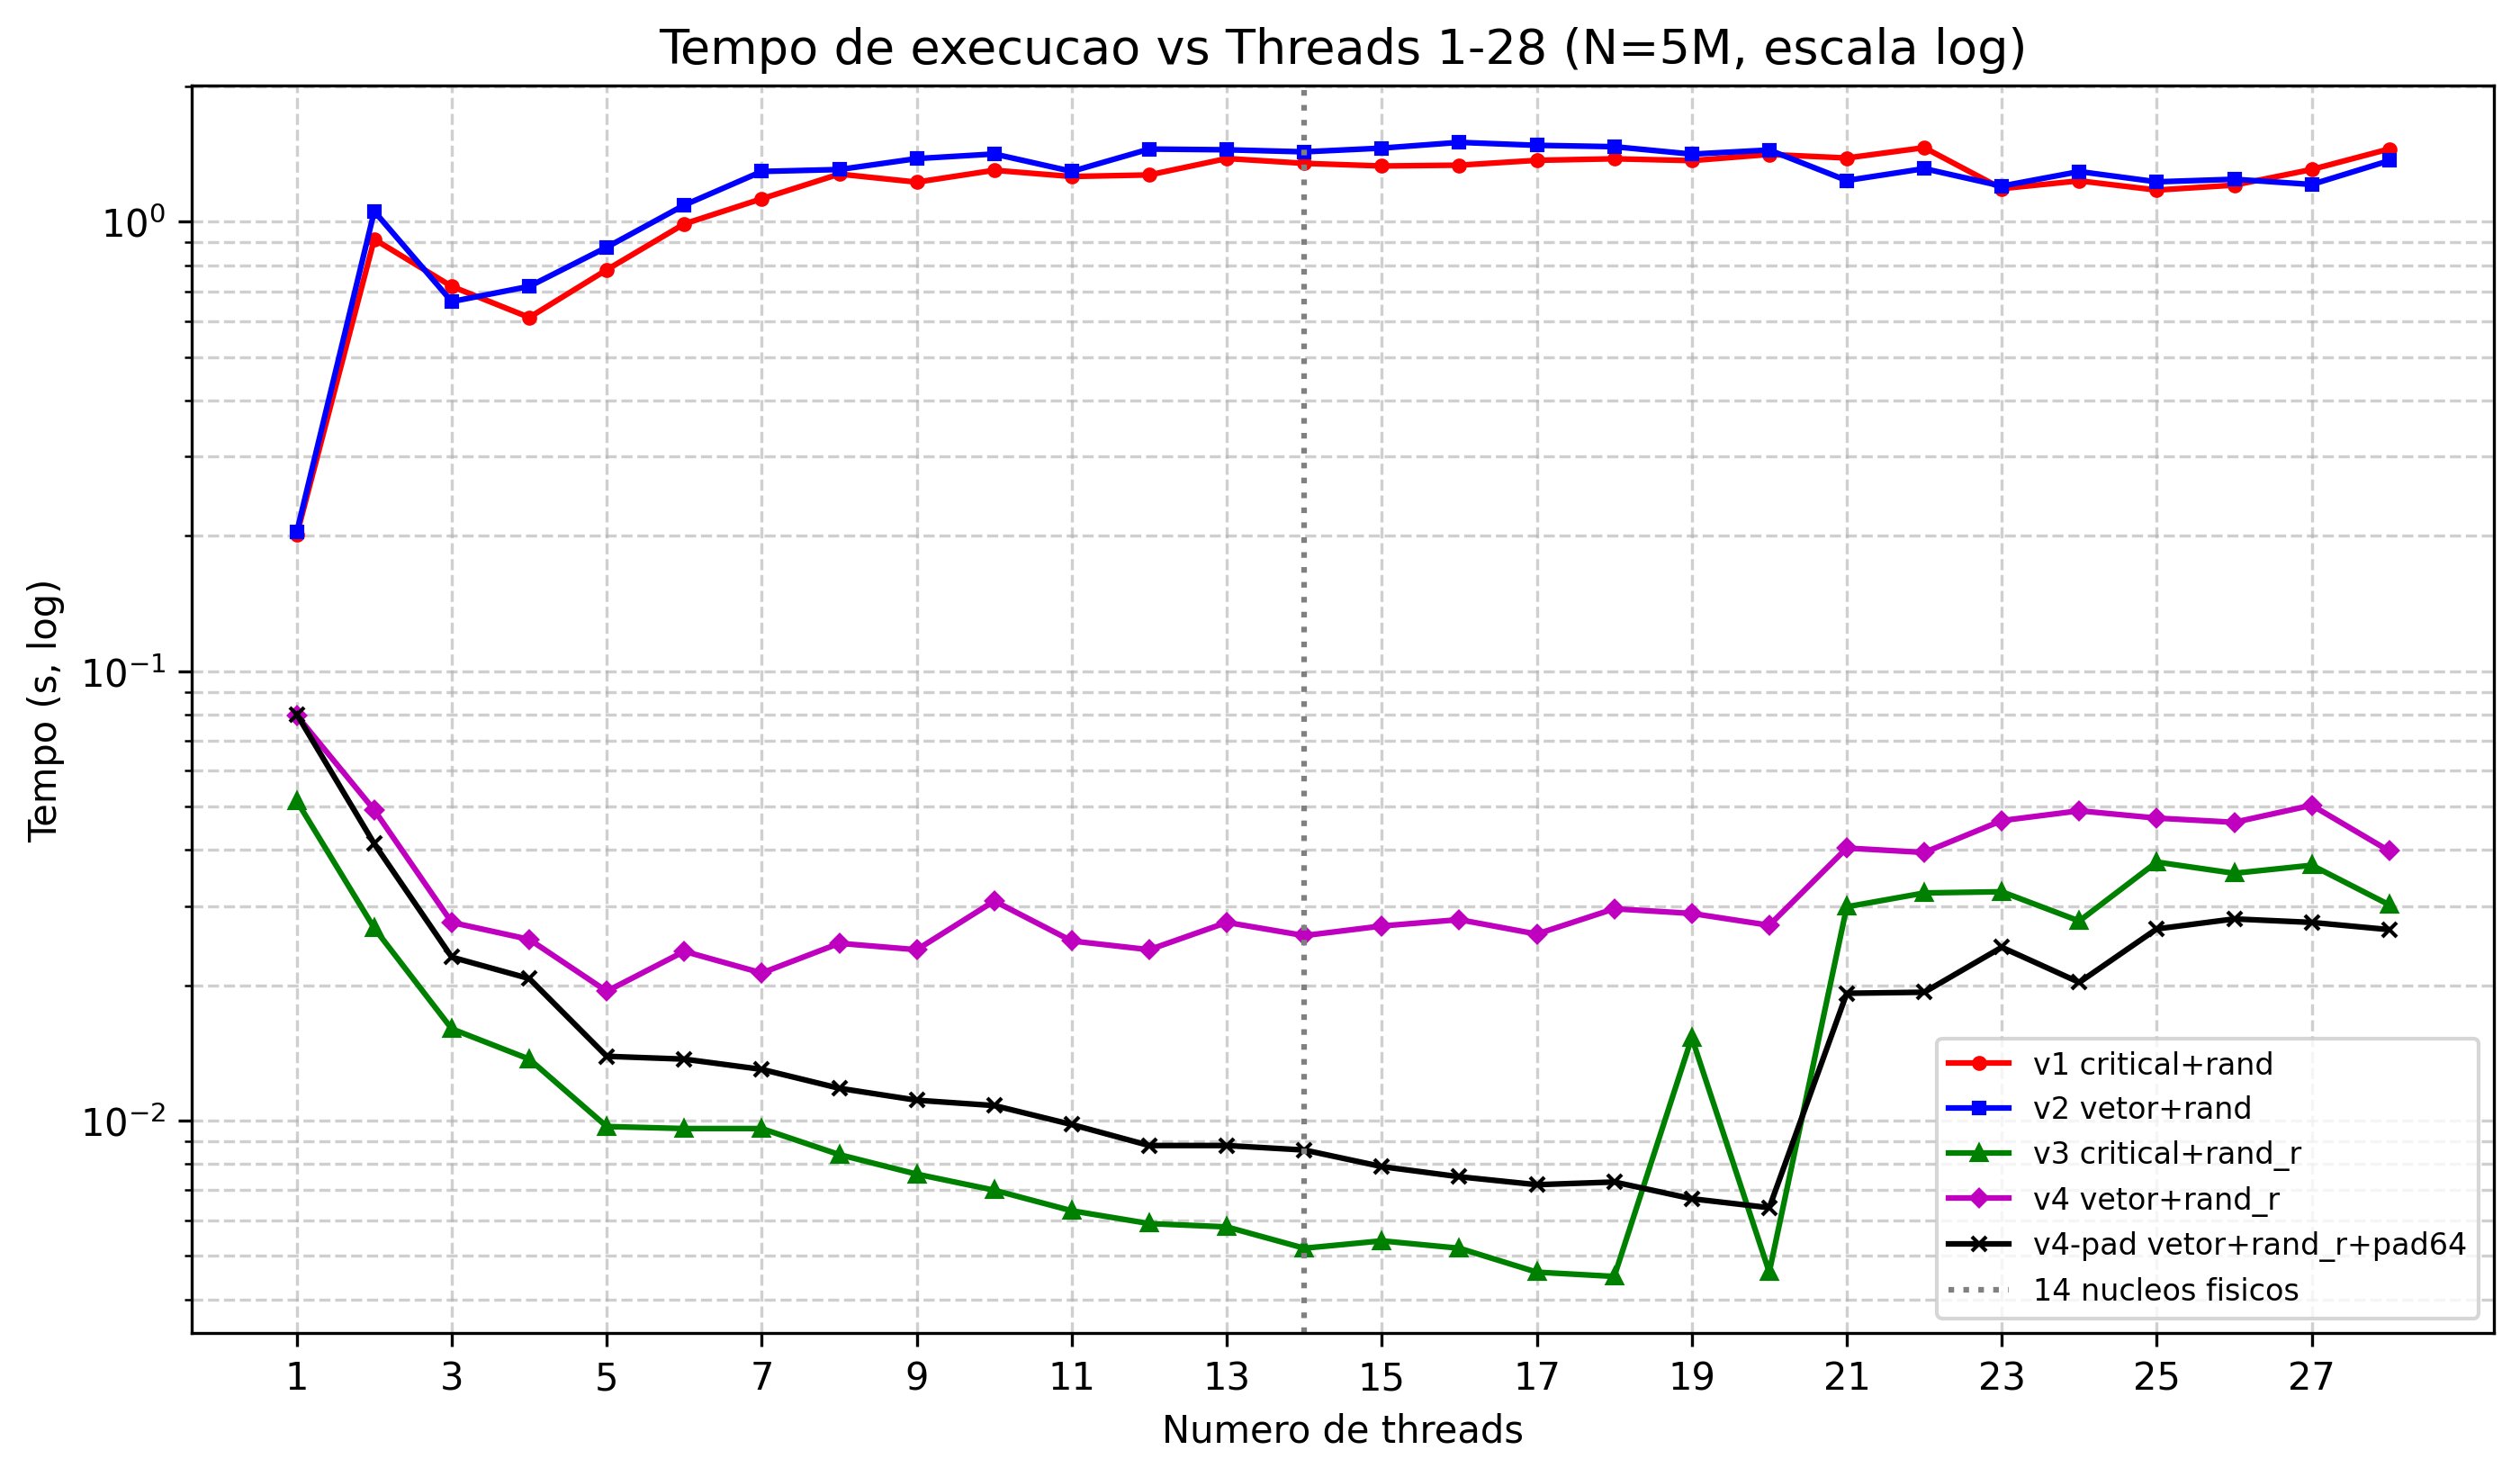
\includegraphics[width=0.9\textwidth]{tempo_execucao_log_plot.png}
\caption{Os mesmos dados em escala logarítmica no eixo $y$. O ganho da versão v3 sobre v1 e v2 fica visível em duas ordens de grandeza, e a separação entre v4 sem e com \textit{padding} aparece em toda a faixa.}
\label{fig:templog}
\end{figure}

\begin{figure}[H]
\centering
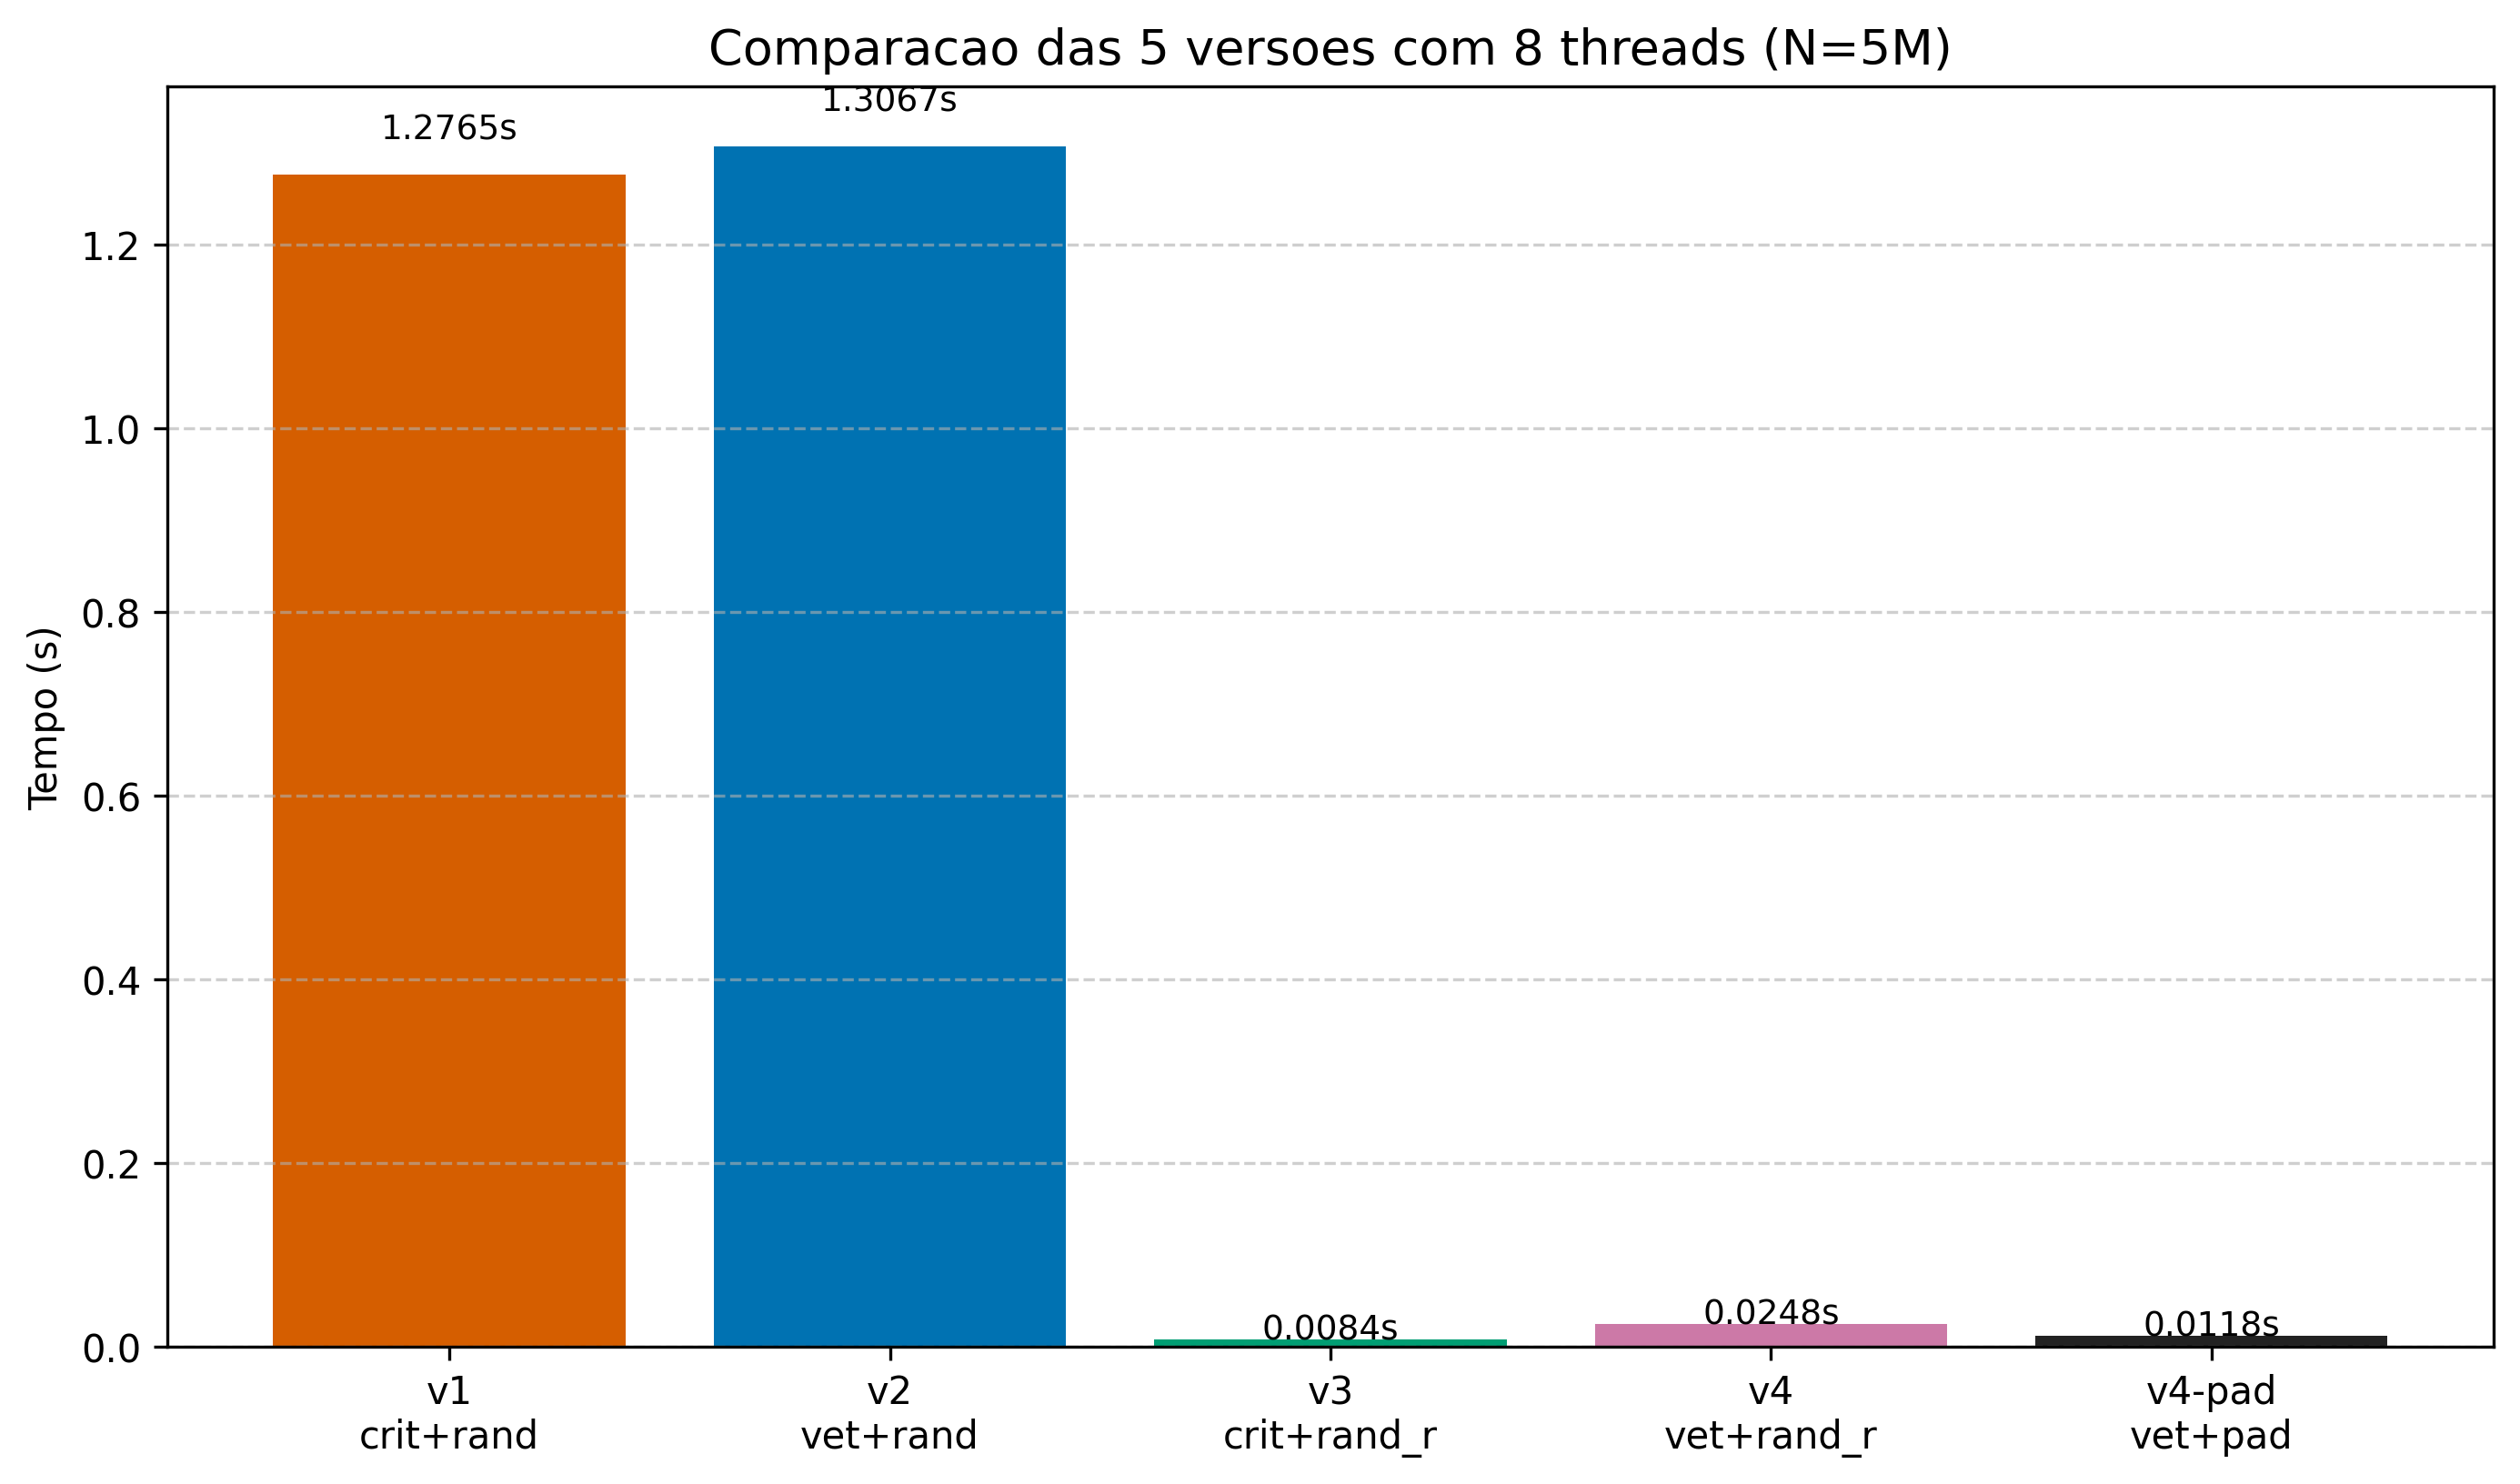
\includegraphics[width=0.9\textwidth]{comparacao_versoes.png}
\caption{Comparação com 8 threads: as versões v1 e v2 são duas ordens de grandeza mais lentas que a v3.}
\label{fig:barra}
\end{figure}

\subsection{Por que v1 e v2 não escalam}

Com 1 thread, v1 e v2 levam cerca de $0{,}20$ s. Com 8 threads, passam de $1{,}3$ s: adicionar threads deixa o programa mais lento. A função \texttt{rand()} tem trava interna e estado global. Todas as threads disputam a mesma linha de cache, e a geração serializa. Mais threads acarretam maior contenção e mais tráfego de coerência no protocolo MESI. O \textit{speedup} fica bem abaixo de $1$. A diferença entre v1 e v2 é pequena porque o gargalo está no gerador, não na soma: trocar \texttt{critical} final por vetor compartilhado não destrava a geração. Além disso, os valores estimados de $\pi$ variam entre execuções com mais de uma thread, sintoma evidente de \textit{data race} no estado de \texttt{rand}.

\subsection{Por que v3 é a mais rápida}

O tempo de v3 cai de $0{,}0514$ s com 1 thread para $0{,}0045$ s com 18 threads, alcançando um ganho de $11{,}4\times$. Até 20 threads, o tempo permanece entre $0{,}004$ s e $0{,}008$ s. Acima de 21 threads, sob efeito de SMT e da virtualização WSL2, sobe para a faixa de $0{,}027$ s a $0{,}037$ s. Cada thread avança sua semente local sem trava e sem tráfego de coerência, e a soma custa apenas $P$ entradas na seção crítica. A ordem de desempenho prevista ($1 > 2 > 3$) confirma-se, e o salto $1 \to 3$ é o mais expressivo por eliminar a serialização das $N$ gerações.

\subsection{Falso compartilhamento visível em v4}

A versão v4 é cerca de $2$ a $5\times$ mais lenta que a v3 na mesma contagem de threads: com 8 threads, consome $0{,}0248$ s contra $0{,}0084$ s; com 14 threads, $0{,}0258$ s contra $0{,}0052$ s. Sem a trava de \texttt{rand} para mascarar a contenção, o ping-pong das linhas de cache contendo o vetor \texttt{hits[tid]++} torna-se dominante. Os $P$ contadores cabem em 1 ou 2 linhas de $64$ B, e cada acerto invalida a linha nos demais núcleos. A variante com \textit{padding} de $64$ B reduz o tempo para $0{,}0118$ s com 8 threads e $0{,}0086$ s com 14 threads (ganho de $2{,}1\times$ a $3{,}0\times$ sobre v4 sem \textit{padding}), confirmando o diagnóstico.

\section{Conclusão}

O fator determinante para o tempo de execução é a geração de números pseudoaleatórios, e não a soma dos acertos. O uso de \texttt{rand()} com estado global inviabiliza a escalabilidade: as versões v1 e v2 desaceleram com mais threads, atingindo cerca de $1{,}3$ s com 8 threads frente a $0{,}20$ s com 1 thread. A substituição por \texttt{rand\_r()} com semente privada destrava a geração e evidencia o custo da soma: v3, com contador privado e redução única ao final, é a mais rápida; v4, com vetor contíguo compartilhado, sofre severamente com falso compartilhamento, efeito mitigado pelo alinhamento e \textit{padding} de $64$ B.

\appendix

\newpage
\section{Código-fonte completo}
\label{apendice:codigos}

\lstinputlisting[caption={v1\_pi\_critical\_rand.c}]{v1_pi_critical_rand.c}

\lstinputlisting[caption={v2\_pi\_vector\_rand.c}]{v2_pi_vector_rand.c}

\lstinputlisting[caption={v3\_pi\_critical\_randr.c}]{v3_pi_critical_randr.c}

\lstinputlisting[caption={v4\_pi\_vector\_randr.c}]{v4_pi_vector_randr.c}

\lstinputlisting[caption={v4\_fix\_pi\_vector\_randr\_pad.c}]{v4_fix_pi_vector_randr_pad.c}

\end{document}
